

\section{Data and Methodology}

\subsection{Data}
The dataset used in this study is sourced from Kaggle and is titled "Emotions Dataset for NLP." This dataset contains 16,000 labeled samples, each expressing one of five distinct emotions: joy, love, surprise, sadness, and anger. The data is structured into two columns: the first representing the text (tweet or statement) and the second representing the associated emotion label. The dataset is highly suitable for training machine learning models designed for emotion detection tasks, as it includes diverse samples of short, real-world text data. The dataset can be accessed via the following link: \href{https://www.kaggle.com/datasets/praveengovi/emotions-dataset-for-nlp/data}{\color{blue}Kaggle Dataset}.

\begin{figure}[H]
    \centering
    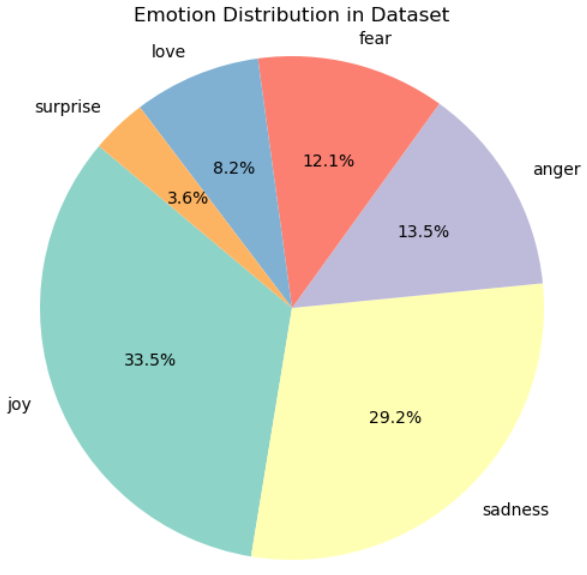
\includegraphics[width=0.6\textwidth]{emotion_pie.png}
    \caption{Percentage distribution of emotions in the dataset.}
    \label{fig:emotion_pie}
\end{figure}

\begin{figure}[H]
    \centering
    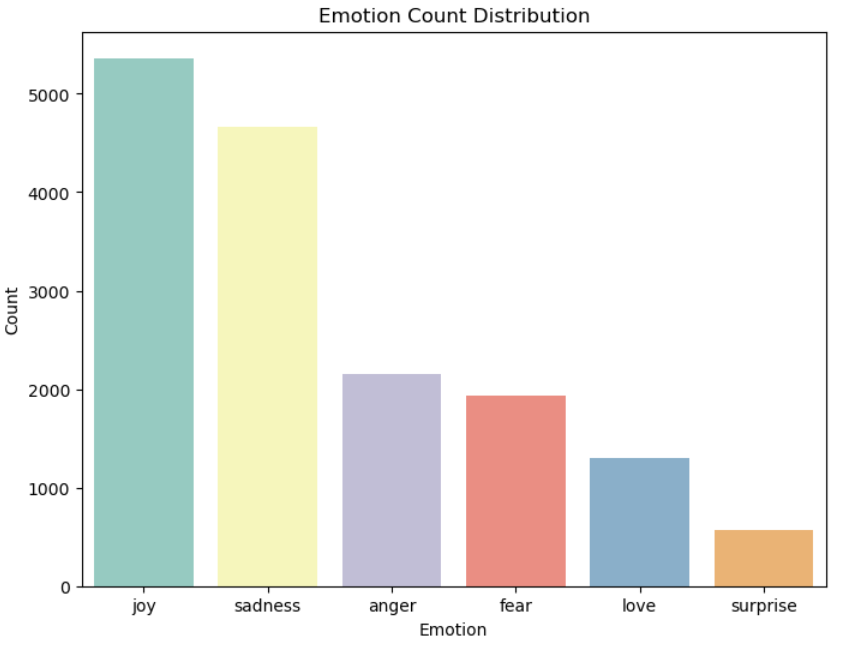
\includegraphics[width=0.6\textwidth]{emotion_bar.png}
    \caption{Count of each emotion in the dataset.}
    \label{fig:emotion_bar}
\end{figure}
The dataset contains six distinct emotions: \textit{joy}, \textit{sadness}, \textit{anger}, \textit{fear}, \textit{love}, and \textit{surprise}. The distribution of these emotions can be visualized in Figure~\ref{fig:emotion_pie}, which shows that \textit{joy} is the most frequent emotion, comprising 33.5\% of the dataset. This is followed by \textit{sadness}, which accounts for 29.2\%, reflecting a notable representation of negative sentiments. Emotions such as \textit{anger} (13.5\%) and \textit{fear} (12.1\%) also have a significant presence, while \textit{love} (8.2\%) is moderately represented. Finally, \textit{surprise} is the least frequent emotion, making up only 3.6\% of the dataset. The bar chart in Figure~\ref{fig:emotion_bar} further highlights the exact counts for each emotion, reinforcing the dominant presence of \textit{joy} and \textit{sadness}, and the relatively rare occurrence of \textit{surprise}.

\begin{figure}[H]
    \centering
    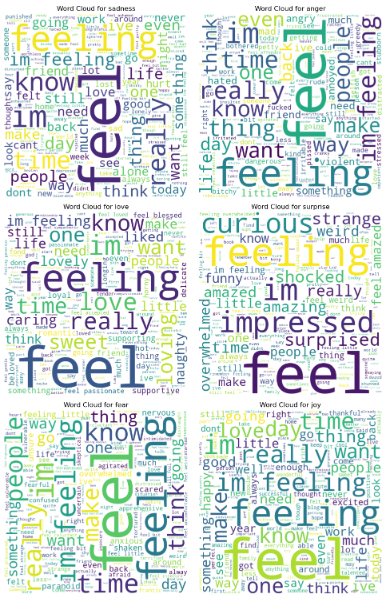
\includegraphics[width=0.6\textwidth]{emotion_cloud.png}
    \caption{Word cloud for the most frequent terms in each emotion.}
    \label{fig:emotion_cloud}
\end{figure}

In addition, Figure~\ref{fig:emotion_cloud} presents a word cloud visualization that showcases the most frequently occurring words in each emotion category. For example, in the \textit{joy} category, words such as \textit{happy}, \textit{excited}, and \textit{great} appear frequently, emphasizing themes of positivity. On the other hand, in the \textit{sadness} category, terms like \textit{loss}, \textit{hurt}, and \textit{tears} dominate, reflecting themes of grief. The \textit{anger} category includes terms such as \textit{mad}, \textit{frustrated}, and \textit{hate}, while the \textit{fear} category features words like \textit{scared} and \textit{nervous}. In the \textit{love} category, words such as \textit{care}, \textit{heart}, and \textit{dear} are more prominent, highlighting affection and compassion. Finally, the \textit{surprise} category shows terms like \textit{shock} and \textit{unexpected}, which represent reactions to unexpected events. Additionally, common words such as \textit{feel} and \textit{feeling} appear across all emotion categories, indicating the strong emotional undertones in the dataset and emphasizing how people often associate emotions with personal feelings.

These visualizations provide crucial insights into the distribution and underlying themes of each emotion in the dataset, offering a comprehensive view of the text data's emotional content.

\section{Methodology}

\begin{figure}[H]
    \centering
    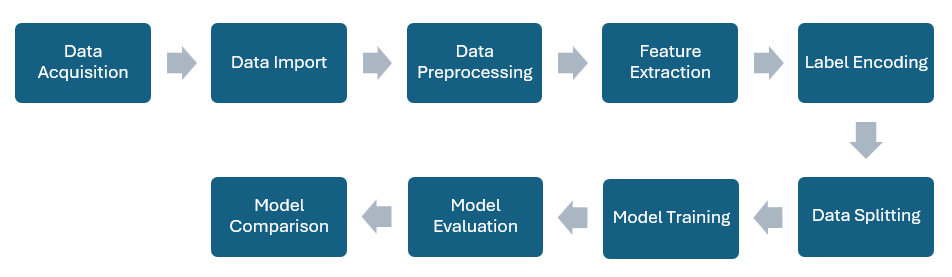
\includegraphics[width=0.8\textwidth]{methodology_flow.png}
    \caption{Flowchart representing the methodology for sentiment analysis.}
    \label{fig:methodology_flow}
\end{figure}

The methodology for this sentiment analysis project is outlined in the flowchart shown in Figure~\ref{fig:methodology_flow}.

The first step in the methodology is data acquisition, where the dataset is obtained from Kaggle. The dataset used in this study is titled "Emotions Dataset for NLP," and it contains textual data labeled with six distinct emotions: joy, sadness, anger, fear, love, and surprise. This dataset serves as the foundation for the sentiment analysis task. Once the dataset is acquired, it is imported into the system using Pandas. The `train.csv` file, which contains 16,000 sentiment samples, is read into a Pandas DataFrame for further processing and analysis.

Data preprocessing is a crucial step to prepare the dataset for analysis. This involves cleaning the text by removing HTML tags, URLs, numbers, special characters, and unwanted patterns using regular expressions (regex). Additionally, stopwords—common words that do not contribute significant meaning, such as "the," "a," "an," etc.—are removed using the NLTK library \cite{opinosis2024stopwords}.

After preprocessing, the text data is converted into numerical features using the TF-IDF (Term Frequency-Inverse Document Frequency) technique. The `TfidfVectorizer` is used to transform the text data into a matrix of TF-IDF features. This method also includes n-grams, specifically unigrams, bigrams, and trigrams, to capture not only individual words but also word pairs and triples, which can provide more context and improve the model's understanding of the relationships between words in the text.

Next, label encoding is performed. Since machine learning models cannot process categorical data directly, the emotion labels (joy, sadness, anger, etc.) are encoded into numerical values using `LabelEncoder`, allowing the model to understand and classify the emotions.

The dataset is then split into training and testing sets. Typically, 80\% of the data is used for training the model, while the remaining 20\% is reserved for testing and evaluation. However, due to an observed imbalance in the emotion classes, stratified sampling was implemented to ensure that the distribution of emotions was preserved in both the training and testing sets. This helps avoid bias that could arise from an uneven distribution of classes. Additionally, upsampling and downsampling techniques were applied to the training dataset to further address class imbalance, ensuring that each emotion class is adequately represented.

Once the data is preprocessed and ready, several machine learning models are trained on the dataset, including Naive Bayes, Logistic Regression, Support Vector Machine (SVM), Random Forest, Artificial Neural Networks (ANN), and XGBoost. Each model is trained using the training set, and its performance is evaluated using the test set.

After training the models, they are evaluated using various performance metrics. These include a classification report showing precision, recall, and F1-score for each emotion class, a confusion matrix illustrating the true positive, true negative, false positive, and false negative counts, and an overall accuracy score for each model on the test data.

The performance of all trained models is then compared. The best performing model is selected based on its accuracy and other evaluation metrics, and it is used for further analysis and potential deployment. Finally, the results are summarized, highlighting the best performing model and its potential application for real-world emotion detection tasks. The selected model is further analyzed to understand its strengths and weaknesses in classifying the emotions.
